\documentclass[12pt,letterpaper,oneside]{book}

\usepackage{7_styles/afitThesis}
\usepackage{7_styles/sf298}
\usepackage{lastpage}
\usepackage{array}
\graphicspath{/5_figures/}
%% myFigures.tex
% A common file to store all figure definitions
%
% In preparing your thesis, one of the first things you should do is
% organize your figures.  Then, one of the last things you'll do is
% reorder your figures so they display where you want them to in the
% text.  Organizing figure definitions in a common files helps:
%
%   1. Write new figures using earlier examples.
%
%   2.  Isolate code and minimize the risk of introducing bugs in the
%   final editing process.  Trust me, moving around just one line of
%   code is easier.
%
%   3.  Reuse figures in other papers.  <=== the best reason!
%
% Note command names can not include numbers and special characters.
%
% To make the file more searchable, use naming conventions that map
% the graphics filename labSetup.jpg to the command name \figlabSetup to the
% figure label fig:labSetup.
% 

%\graphicspath{/5_figures/}
%%%%%%%%%%%%%%%%%%%%%%%%%%%%%%%%%%%%%%%%%%%
\newcommand{\figTransporationConsortium}{\begin{figure}[h]
    \vspace{20pt}
    \begin{center}
    	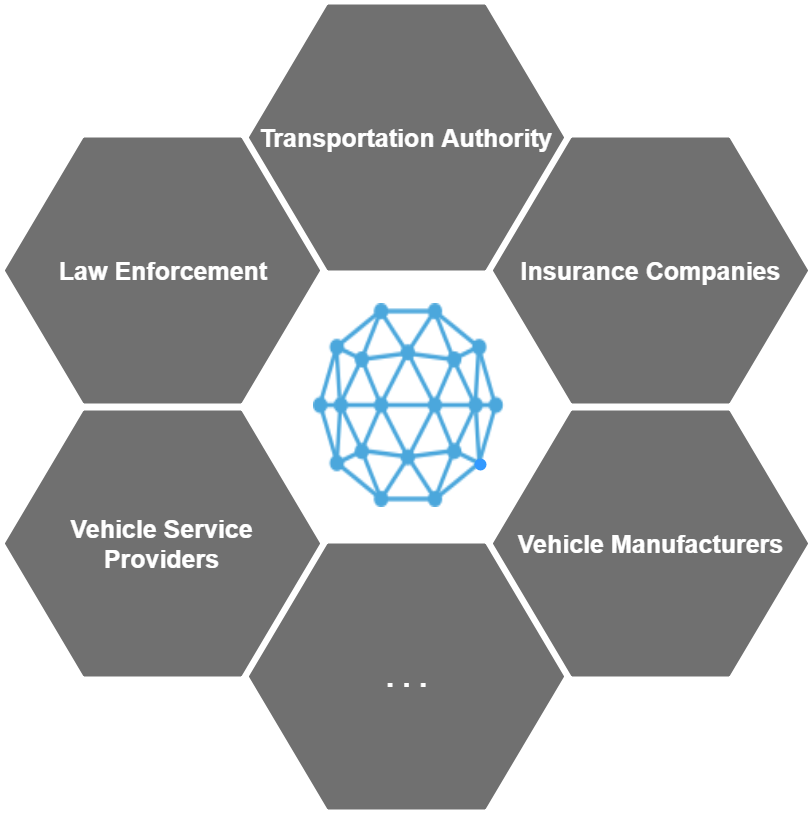
\includegraphics[width=250pt]{5_figures/ConsortiumFigure.png}
    	\caption{Transportation Infrastructure Consortium Members} \label{figTransporationConsortium}
    \end{center}
\end{figure}
}


\newcommand{\figtitlePage}{\begin{figure}[tbp]
    \vspace{20pt}
    \begin{center}
        
\includegraphics[width=2in]{5_figures/afitlogo}
        \caption{Enter student data in titlePage.tex to customize the document's first pages.}
     \label{fig:titlePage}
 \end{center}
\end{figure}
}

\newglossary*{symbol}{Symbols}
\makeglossaries
\loadglsentries{4_support/definitions}
\loadglsentries[acronym]{4_support/acronyms}
\loadglsentries{4_support/symbols}

%% Customize your document with your personal information
%% First, comment out the appropriate document type
\afitthesis %%default
% \afitreport
% \dissertation
% \prospectus

\author{First MI. Lastname}
\rank{Rank, USAF} 

\docdesignator{AFIT-ENG-MS-XX-M-XXX}
\department{Department of Electrical and Computer Engineering}
\graduationdate{March 201X}

\flytitle{THIS IS THE TITLE} 
\title{\MakeUppercase{THIS IS THE TITLE}}
                             % Note, if you use \MakeUppercase to put
                             % the title in all uppercase as the style
                             % guide demands, understand that the
                             % command does not allow page breaks ``\\'' 
                             % within its brackets.
\previousdegrees{B.S.}
\acdegree{Master of Science in XXXXXXX Engineering}

\committee{{First Last, Ph.D.\\Chair},
           {First Last, Ph.D., P.E.\\Member},
           {First Last, Ph.D.\\Member}}

\address{2950 Hobson Way\\ Air Force Institute of Technology \\
Wright-Patterson AFB, OH 45433}

\distribution{DISTRIBUTION STATEMENT A\\[-10pt]
\MakeUppercase{Approved for Public Release; distribution unlimited.}
} 

\disclaimer{The views expressed in this document are those of the
author and do not reflect the official policy or position of the
United States Air Force, the United States Department of Defense or
the United States Government.  This material is declared a work of the
U.S. Government and is not subject to copyright protection in the
United States.}

% International students may consider using the following disclaimer
% statement: \dislaimer{The views expressed in this document are those
% of the author(s) and do not reflect the official policy or position
% of the United States Air Force, Department of Defense, United States
% Government, the corresponding agencies of any other government,
% NATO, or any other defense organization.}



\begin{document}

\frontmatter
	\flyleaf                        
	\disclaimerpage                 
	\titlepageAFIT                      
	\committeepage  
	\begin{abstract}
Lorem ipsum dolor sit amet, consectetur adipiscing elit. Vestibulum convallis malesuada enim ut fermentum. Curabitur magna libero, tempus vitae orci in, malesuada scelerisque orci. Sed ac orci blandit, suscipit mauris sed, feugiat ipsum. Aenean vitae neque et metus feugiat laoreet. In feugiat eros ut tempus congue. Suspendisse gravida pellentesque tortor, quis auctor massa aliquam at. Class aptent taciti sociosqu ad litora torquent per conubia nostra, per inceptos himenaeos. Cras dictum est sem, sit amet ultrices lacus auctor vitae. Curabitur tristique dolor nec est auctor tempus.
\end{abstract}
    \begin{dedication}
 
Sed ac orci blandit, suscipit mauris sed, feugiat ipsum. Aenean vitae neque et metus feugiat laoreet.

\end{dedication}
    \begin{acknowledgements}
Lorem ipsum dolor sit amet, consectetur adipiscing elit. Vestibulum convallis malesuada enim ut fermentum. Curabitur magna libero, tempus vitae orci in, malesuada scelerisque orci. Sed ac orci blandit, suscipit mauris sed, feugiat ipsum. Aenean vitae neque et metus feugiat laoreet. 

In feugiat eros ut tempus congue. Suspendisse gravida pellentesque tortor, quis auctor massa aliquam at. Class aptent taciti sociosqu ad litora torquent per conubia nostra, per inceptos himenaeos. Cras dictum est sem, sit amet ultrices lacus auctor vitae. Curabitur tristique dolor nec est auctor tempus.

\end{acknowledgements}




    \tableofcontents
    \listoffigures
    \listoftables
    \listofalgorithms
    \listofabbreviations
    
\mainmatter
	\chapter{Introduction}
    	\section{Background and Motivation}
    Lorem ipsum dolor sit amet, consectetur adipiscing elit. Mauris nec nunc nisi. Aenean efficitur massa quam, dictum ullamcorper sapien maximus sit amet. Sed rhoncus commodo velit nec vestibulum. Integer nec nisi quis urna bibendum pharetra. Etiam posuere nunc non erat consectetur, quis aliquet leo aliquam. Aenean quis mi in enim volutpat fermentum. Vestibulum dignissim suscipit posuere. Integer lacinia non dui eu efficitur. Donec scelerisque libero condimentum imperdiet finibus. Morbi vel finibus tellus. Integer malesuada mattis dignissim. Etiam a enim a mi rhoncus eleifend quis sit amet purus.

\section{Problem Statement}
    Fusce bibendum tortor ut eros viverra imperdiet. Quisque quis arcu iaculis, volutpat metus at, semper ex. Nam ac hendrerit enim, eget fringilla urna. Curabitur quis commodo nisl, in rutrum enim. Nunc ut elit porta, volutpat mauris eget, pulvinar nisi. Proin ullamcorper accumsan erat nec dignissim. Curabitur ante lacus, sollicitudin a sapien vitae, maximus sodales nulla. Sed quis congue odio. Sed quis dui suscipit, vulputate risus id, rhoncus nisl. Pellentesque arcu mauris, egestas et urna at, rhoncus tincidunt ipsum. Sed ex magna, ornare id tellus in, scelerisque iaculis tortor.
    
\section{Examples}
\subsection{References from BibTex file}
    Use cite command and the identifier of the entry as the parameter. Bibliography is automatically generated. If doing auto-import from Mendeley, url accessed date will not be included.\\
    Single Ref:    \cite{NHTSA2010OdometerFraud} \\
    Multi Ref:     \cite{NHTSA2010OdometerFraud,NHTSA2010OdometerFraud}\\
\subsection{Acronyms}
    To use acronyms, add the acronym and definition to the acronyms.tex file under 4\_support folder.
    
    Use the following commands when using acronyms gls (regular) and glspl to show the plural form (automatically appends an `s' at the end). By using these commands, your acronyms list will be automatically generated.
    Examples:
    \begin{enumerate}
        \item  \gls{af}
        \item  \gls{af}
        \item  \glspl{af}
    \end{enumerate}
    
    
\subsection{Tables}
    Tables can be defined in the tables.tex folder and referenced here by command name or within the chapter file as follows:
    \begin{table}[!h]
	\centering
	\small
	\rowcolors{2}{gray!25}{white}
	\caption{DLT Alternatives.}\label{table:DLTComparison}
	\begin{tabular}{>{\centering\arraybackslash}p{1.9cm}>{\centering\arraybackslash}p{1.9cm}>{\centering\arraybackslash}p{1.9cm}>{\centering\arraybackslash}p{2.2cm}>{\centering\arraybackslash}p{2.2cm}>{\centering\arraybackslash}p{2cm}}
		\toprule
		\textbf{Name}&\textbf{Executable}&\textbf{API/SDK Ready}&\textbf{Permissioned}&\textbf{Smart Contracts}&\textbf{\$0 License Cost} \\
		\midrule
		Tendermint & \checkmark  & \checkmark  & &  & \checkmark \\
		MultiChain & \checkmark & \checkmark& \checkmark &\checkmark  &  \\
		Hyperledger Fabric & \checkmark & \checkmark& \checkmark &  \checkmark & \checkmark \\
		\bottomrule
	\end{tabular}
    \end{table}
    
\subsection{Figures}
    Figures can be defined in the figures.tex file and referenced here by command name or within the chapter file as follows:
    \figtitlePage
    
    \begin{figure}[tbp]
        \vspace{20pt}
        \begin{center}
            
\includegraphics[width=2in]{5_figures/afitlogo}
            \caption{Enter student data in titlePage.tex to customize the document's first pages.}
         \label{fig:titlePageTwo}
     \end{center}
    \end{figure}

\subsection{Algorithms}
    Example of algorithmic package for algorithms.
    
    \begin{algorithm}[!h]
        	\caption{Road Event Witnessed Data Transaction}
        	\begin{algorithmic}[1]
        		\State //tx $\leftarrow$ \{sourceId, eventId, WitnessedData\}
        		\If{tx.WitnessedData.length$>0$ \& SensorExists(tx.sourceId) \& IsValid(tx)} %RoadEventExists(tx.eventId)
        		\State $wd \leftarrow WitnessedData(tx)$
        		\State $WitnessedDataRegistry.add(wd)$
        		\State emit(WitnessedDataSubmitted)
        		\Else
        		\State emit(InvalidWitnessedDataTx)
        		\EndIf
        	\end{algorithmic}
        	\label{algo:submitWitness}
        \end{algorithm}

\subsection{Appendices}
    Defined in 2\_main/appendix and imported to main.tex file. Reference Appendix~\ref{appendix:configuration}.


    	
    \chapter{Background and Related Work}
    	\section{Overview}
    Lorem ipsum dolor sit amet, consectetur adipiscing elit. Mauris nec nunc nisi. Aenean efficitur massa quam, dictum ullamcorper sapien maximus sit amet. Sed rhoncus commodo velit nec vestibulum. Integer nec nisi quis urna bibendum pharetra. Etiam posuere nunc non erat consectetur, quis aliquet leo aliquam. Aenean quis mi in enim volutpat fermentum. Vestibulum dignissim suscipit posuere. Integer lacinia non dui eu efficitur. Donec scelerisque libero condimentum imperdiet finibus. Morbi vel finibus tellus. Integer malesuada mattis dignissim. Etiam a enim a mi rhoncus eleifend quis sit amet purus.
    
\section{Summary}
   Fusce bibendum tortor ut eros viverra imperdiet. Quisque quis arcu iaculis, volutpat metus at, semper ex. Nam ac hendrerit enim, eget fringilla urna. Curabitur quis commodo nisl, in rutrum enim. Nunc ut elit porta, volutpat mauris eget, pulvinar nisi. Proin ullamcorper accumsan erat nec dignissim. Curabitur ante lacus, sollicitudin a sapien vitae, maximus sodales nulla. Sed quis congue odio. Sed quis dui suscipit, vulputate risus id, rhoncus nisl. Pellentesque arcu mauris, egestas et urna at, rhoncus tincidunt ipsum. Sed ex magna, ornare id tellus in, scelerisque iaculis tortor.
    
    \chapter{Design}
    	\section{Overview}
   Lorem ipsum dolor sit amet, consectetur adipiscing elit. Mauris nec nunc nisi. Aenean efficitur massa quam, dictum ullamcorper sapien maximus sit amet. Sed rhoncus commodo velit nec vestibulum. Integer nec nisi quis urna bibendum pharetra. Etiam posuere nunc non erat consectetur, quis aliquet leo aliquam. Aenean quis mi in enim volutpat fermentum. Vestibulum dignissim suscipit posuere. Integer lacinia non dui eu efficitur. Donec scelerisque libero condimentum imperdiet finibus. Morbi vel finibus tellus. Integer malesuada mattis dignissim. Etiam a enim a mi rhoncus eleifend quis sit amet purus.

        
\section{Summary}
  Fusce bibendum tortor ut eros viverra imperdiet. Quisque quis arcu iaculis, volutpat metus at, semper ex. Nam ac hendrerit enim, eget fringilla urna. Curabitur quis commodo nisl, in rutrum enim. Nunc ut elit porta, volutpat mauris eget, pulvinar nisi. Proin ullamcorper accumsan erat nec dignissim. Curabitur ante lacus, sollicitudin a sapien vitae, maximus sodales nulla. Sed quis congue odio. Sed quis dui suscipit, vulputate risus id, rhoncus nisl. Pellentesque arcu mauris, egestas et urna at, rhoncus tincidunt ipsum. Sed ex magna, ornare id tellus in, scelerisque iaculis tortor.
    
    \chapter{Experimental Scenarios}
    	Lorem ipsum dolor sit amet, consectetur adipiscing elit. Mauris nec nunc nisi. Aenean efficitur massa quam, dictum ullamcorper sapien maximus sit amet. Sed rhoncus commodo velit nec vestibulum. Integer nec nisi quis urna bibendum pharetra. Etiam posuere nunc non erat consectetur, quis aliquet leo aliquam. Aenean quis mi in enim volutpat fermentum. Vestibulum dignissim suscipit posuere. Integer lacinia non dui eu efficitur. Donec scelerisque libero condimentum imperdiet finibus. Morbi vel finibus tellus. Integer malesuada mattis dignissim. Etiam a enim a mi rhoncus eleifend quis sit amet purus.

Fusce bibendum tortor ut eros viverra imperdiet. Quisque quis arcu iaculis, volutpat metus at, semper ex. Nam ac hendrerit enim, eget fringilla urna. Curabitur quis commodo nisl, in rutrum enim. Nunc ut elit porta, volutpat mauris eget, pulvinar nisi. Proin ullamcorper accumsan erat nec dignissim. Curabitur ante lacus, sollicitudin a sapien vitae, maximus sodales nulla. Sed quis congue odio. Sed quis dui suscipit, vulputate risus id, rhoncus nisl. Pellentesque arcu mauris, egestas et urna at, rhoncus tincidunt ipsum. Sed ex magna, ornare id tellus in, scelerisque iaculis tortor.

Donec nisi tellus, interdum ac imperdiet eu, facilisis quis diam. Suspendisse dignissim lacinia ex. Phasellus eu mauris id elit iaculis ornare. Quisque nec magna id tortor porta efficitur consequat eget tortor. Curabitur convallis mi metus, vitae iaculis purus convallis non. Duis eleifend imperdiet placerat. Nulla facilisi. Donec eu diam metus. Cras nec erat quis ligula auctor finibus et non nisl. Vivamus sit amet congue nulla, ut pulvinar ante. Duis enim ligula, efficitur et mauris et, accumsan vehicula risus. Aliquam ultricies neque ac libero ullamcorper, eu placerat neque efficitur.

Nullam malesuada auctor mauris, tempor ultricies leo. Cras lacus tortor, dignissim vel dolor nec, ultrices pellentesque libero. Donec eget orci sem. Sed sed purus convallis, blandit nibh at, porta lectus. Sed ac ante erat. Praesent a felis consequat, commodo dolor at, pulvinar ligula. Nunc dapibus odio et libero semper, nec euismod leo dapibus. In et nunc porttitor, cursus eros ac, molestie eros. Nam mattis aliquam metus, quis ornare nibh. Nam accumsan, lacus vel molestie scelerisque, magna mauris pharetra libero, ut viverra urna ex in tortor. Sed tincidunt nec neque consequat interdum. Aliquam ligula justo, interdum in blandit in, fringilla sed neque.

Nullam semper at lectus et egestas. Proin facilisis turpis ipsum, sed molestie nisi varius eu. Quisque sed enim vel quam dictum tempor. Nulla varius, justo at bibendum pharetra, ligula felis condimentum neque, nec posuere sem risus ut justo. Vestibulum vel convallis urna, at porttitor velit. Suspendisse eros dolor, convallis accumsan iaculis et, mollis ac eros. Cras sit amet nibh eget lacus dapibus condimentum. Quisque ligula massa, ullamcorper in dapibus eget, mattis ac mi. Cras sit amet nibh vel elit egestas vulputate. Donec sed tortor pulvinar, accumsan enim sed, imperdiet risus. Nunc quis sagittis elit. Curabitur elementum, lorem ut fringilla tempor, augue tortor imperdiet massa, in imperdiet dui felis id nunc. Duis accumsan velit vitae augue tincidunt, in blandit lorem fermentum. Praesent commodo mattis blandit.
    
    \chapter{Observations and Analysis}
    		Lorem ipsum dolor sit amet, consectetur adipiscing elit. Mauris nec nunc nisi. Aenean efficitur massa quam, dictum ullamcorper sapien maximus sit amet. Sed rhoncus commodo velit nec vestibulum. Integer nec nisi quis urna bibendum pharetra. Etiam posuere nunc non erat consectetur, quis aliquet leo aliquam. Aenean quis mi in enim volutpat fermentum. Vestibulum dignissim suscipit posuere. Integer lacinia non dui eu efficitur. Donec scelerisque libero condimentum imperdiet finibus. Morbi vel finibus tellus. Integer malesuada mattis dignissim. Etiam a enim a mi rhoncus eleifend quis sit amet purus.

Fusce bibendum tortor ut eros viverra imperdiet. Quisque quis arcu iaculis, volutpat metus at, semper ex. Nam ac hendrerit enim, eget fringilla urna. Curabitur quis commodo nisl, in rutrum enim. Nunc ut elit porta, volutpat mauris eget, pulvinar nisi. Proin ullamcorper accumsan erat nec dignissim. Curabitur ante lacus, sollicitudin a sapien vitae, maximus sodales nulla. Sed quis congue odio. Sed quis dui suscipit, vulputate risus id, rhoncus nisl. Pellentesque arcu mauris, egestas et urna at, rhoncus tincidunt ipsum. Sed ex magna, ornare id tellus in, scelerisque iaculis tortor.

Donec nisi tellus, interdum ac imperdiet eu, facilisis quis diam. Suspendisse dignissim lacinia ex. Phasellus eu mauris id elit iaculis ornare. Quisque nec magna id tortor porta efficitur consequat eget tortor. Curabitur convallis mi metus, vitae iaculis purus convallis non. Duis eleifend imperdiet placerat. Nulla facilisi. Donec eu diam metus. Cras nec erat quis ligula auctor finibus et non nisl. Vivamus sit amet congue nulla, ut pulvinar ante. Duis enim ligula, efficitur et mauris et, accumsan vehicula risus. Aliquam ultricies neque ac libero ullamcorper, eu placerat neque efficitur.

Nullam malesuada auctor mauris, tempor ultricies leo. Cras lacus tortor, dignissim vel dolor nec, ultrices pellentesque libero. Donec eget orci sem. Sed sed purus convallis, blandit nibh at, porta lectus. Sed ac ante erat. Praesent a felis consequat, commodo dolor at, pulvinar ligula. Nunc dapibus odio et libero semper, nec euismod leo dapibus. In et nunc porttitor, cursus eros ac, molestie eros. Nam mattis aliquam metus, quis ornare nibh. Nam accumsan, lacus vel molestie scelerisque, magna mauris pharetra libero, ut viverra urna ex in tortor. Sed tincidunt nec neque consequat interdum. Aliquam ligula justo, interdum in blandit in, fringilla sed neque.

Nullam semper at lectus et egestas. Proin facilisis turpis ipsum, sed molestie nisi varius eu. Quisque sed enim vel quam dictum tempor. Nulla varius, justo at bibendum pharetra, ligula felis condimentum neque, nec posuere sem risus ut justo. Vestibulum vel convallis urna, at porttitor velit. Suspendisse eros dolor, convallis accumsan iaculis et, mollis ac eros. Cras sit amet nibh eget lacus dapibus condimentum. Quisque ligula massa, ullamcorper in dapibus eget, mattis ac mi. Cras sit amet nibh vel elit egestas vulputate. Donec sed tortor pulvinar, accumsan enim sed, imperdiet risus. Nunc quis sagittis elit. Curabitur elementum, lorem ut fringilla tempor, augue tortor imperdiet massa, in imperdiet dui felis id nunc. Duis accumsan velit vitae augue tincidunt, in blandit lorem fermentum. Praesent commodo mattis blandit.
    
    \chapter{Conclusion}
    	Lorem ipsum dolor sit amet, consectetur adipiscing elit. Mauris nec nunc nisi. Aenean efficitur massa quam, dictum ullamcorper sapien maximus sit amet. Sed rhoncus commodo velit nec vestibulum. Integer nec nisi quis urna bibendum pharetra. Etiam posuere nunc non erat consectetur, quis aliquet leo aliquam. Aenean quis mi in enim volutpat fermentum. Vestibulum dignissim suscipit posuere. Integer lacinia non dui eu efficitur. Donec scelerisque libero condimentum imperdiet finibus. Morbi vel finibus tellus. Integer malesuada mattis dignissim. Etiam a enim a mi rhoncus eleifend quis sit amet purus.

Fusce bibendum tortor ut eros viverra imperdiet. Quisque quis arcu iaculis, volutpat metus at, semper ex. Nam ac hendrerit enim, eget fringilla urna. Curabitur quis commodo nisl, in rutrum enim. Nunc ut elit porta, volutpat mauris eget, pulvinar nisi. Proin ullamcorper accumsan erat nec dignissim. Curabitur ante lacus, sollicitudin a sapien vitae, maximus sodales nulla. Sed quis congue odio. Sed quis dui suscipit, vulputate risus id, rhoncus nisl. Pellentesque arcu mauris, egestas et urna at, rhoncus tincidunt ipsum. Sed ex magna, ornare id tellus in, scelerisque iaculis tortor.

Donec nisi tellus, interdum ac imperdiet eu, facilisis quis diam. Suspendisse dignissim lacinia ex. Phasellus eu mauris id elit iaculis ornare. Quisque nec magna id tortor porta efficitur consequat eget tortor. Curabitur convallis mi metus, vitae iaculis purus convallis non. Duis eleifend imperdiet placerat. Nulla facilisi. Donec eu diam metus. Cras nec erat quis ligula auctor finibus et non nisl. Vivamus sit amet congue nulla, ut pulvinar ante. Duis enim ligula, efficitur et mauris et, accumsan vehicula risus. Aliquam ultricies neque ac libero ullamcorper, eu placerat neque efficitur.

Nullam malesuada auctor mauris, tempor ultricies leo. Cras lacus tortor, dignissim vel dolor nec, ultrices pellentesque libero. Donec eget orci sem. Sed sed purus convallis, blandit nibh at, porta lectus. Sed ac ante erat. Praesent a felis consequat, commodo dolor at, pulvinar ligula. Nunc dapibus odio et libero semper, nec euismod leo dapibus. In et nunc porttitor, cursus eros ac, molestie eros. Nam mattis aliquam metus, quis ornare nibh. Nam accumsan, lacus vel molestie scelerisque, magna mauris pharetra libero, ut viverra urna ex in tortor. Sed tincidunt nec neque consequat interdum. Aliquam ligula justo, interdum in blandit in, fringilla sed neque.

Nullam semper at lectus et egestas. Proin facilisis turpis ipsum, sed molestie nisi varius eu. Quisque sed enim vel quam dictum tempor. Nulla varius, justo at bibendum pharetra, ligula felis condimentum neque, nec posuere sem risus ut justo. Vestibulum vel convallis urna, at porttitor velit. Suspendisse eros dolor, convallis accumsan iaculis et, mollis ac eros. Cras sit amet nibh eget lacus dapibus condimentum. Quisque ligula massa, ullamcorper in dapibus eget, mattis ac mi. Cras sit amet nibh vel elit egestas vulputate. Donec sed tortor pulvinar, accumsan enim sed, imperdiet risus. Nunc quis sagittis elit. Curabitur elementum, lorem ut fringilla tempor, augue tortor imperdiet massa, in imperdiet dui felis id nunc. Duis accumsan velit vitae augue tincidunt, in blandit lorem fermentum. Praesent commodo mattis blandit.
    
    \begin{appendix}
        \chapter{Appendix Title One}
            \label{appendix:configuration}
           \begin{lstlisting}[language=python]
# AFIT Transportation Network Cryto Generation Configuration
# Updated By: Luis A. Cintron

# -----------------------------------------------------------
# "OrdererOrgs" - Definition of orgs managing orderer nodes
# -----------------------------------------------------------
OrdererOrgs:
  - Name: Orderer
    Domain: orderer.afit.edu
    Specs:
      - Hostname: orderer1
        CommonName: orderer1.afit.edu
        SANS:
          - 192.168.64.21
      - Hostname: orderer2
        CommonName: orderer2.afit.edu
        SANS:
          - 192.168.64.22
      - Hostname: orderer3
        CommonName: orderer3.afit.edu
        SANS:
          - 192.168.64.23

\end{lstlisting}
        \begin{landscape}
        \chapter{Appendix Title Two}
            \label{appendix:performanceDataOutput}
            \tiny
%
\begin{longtable}{p{0.7cm} *{2}{p{0.4cm}} p{1.2cm} p{0.5cm} *{2}{p{1.3cm}} p{0.4cm} *{3}{p{1.1cm}} *{10}{p{0.4cm}}}
    		\toprule
            Scenario & Req No. & Block &Req Submit Time&Req/s&Avg Total Req Time&Total Time Elapsed&Successful&Timeout Error&HLF Error&Total Errors&Avg TPS & Peak TPS & Total Blocks & Avg BPS & Peak BPS & Avg TPB & Peak TPB & Min TPB & Total Tx & Total Time \\
            \midrule
            1&10&6&0.902&11.0864745&1.1162&1.576&10&0&0&0&5&6&1&1&1&10&10&10&10&1\\
            2&10&7&0.903&11.07419712&0.901&1.36&10&0&0&0&5&7&1&1&1&10&10&10&10&1\\
            3&10&8&0.902&11.0864745&0.9405&1.395&10&0&0&0&5&7&1&1&1&10&10&10&10&1\\
            4&20&9&0.951&21.03049422&1.56615&2.505&20&0&0&0&10&14&2&1&1&10&10&10&20&1\\
            5&20&11&0.951&21.03049422&1.4166&2.532&20&0&0&0&10&16&2&1&1&10&15&5&20&1\\
            6&20&13&0.951&21.03049422&1.66775&2.654&20&0&0&0&10&17&2&1&1&10&11&9&20&1\\
            7&30&15&0.968&30.99173554&2.2277&2.99&30&0&0&0&15&28&2&2&2&15&20&10&30&1\\
            8&30&17&0.968&30.99173554&2.139566667&2.935&30&0&0&0&15&22&2&2&2&15&19&11&30&1\\
            9&30&19&0.968&30.99173554&2.1227&2.721&30&0&0&0&15&16&2&2&2&15&25&5&30&1\\
            10&40&21&0.976&40.98360656&2.67125&3.245&40&0&0&0&20&33&2&2&2&20&35&5&40&1\\
            11&40&23&0.977&40.94165814&2.978225&3.731&40&0&0&0&20&31&2&2&2&20&27&13&40&1\\
            12&40&25&0.978&40.8997955&2.962325&3.612&40&0&0&0&20&28&2&2&2&20&32&8&40&1\\
            13&50&27&0.981&50.96839959&3.344&3.894&50&0&0&0&25&34&2&2&2&25&47&3&50&1\\
            14&50&29&0.983&50.8646999&3.4654&4.104&50&0&0&0&25&49&2&1&1&25&43&7&50&1\\
            15&50&31&0.982&50.91649695&3.3642&3.903&50&0&0&0&25&39&2&2&2&25&47&3&50&1\\
            16&60&33&0.986&60.85192698&3.927666667&4.751&60&0&0&0&30&39&2&1&1&30&40&20&60&1\\
            17&60&35&0.987&60.79027356&4.76945&5.74&60&0&0&0&30&38&3&1.5&2&20&45&4&60&1\\
            18&60&38&0.986&60.85192698&3.830566667&4.782&60&0&0&0&30&50&2&1&1&30&30&30&60&1\\
            19&70&40&0.988&70.85020243&4.556257143&5.589&70&0&0&0&35&67&3&3&3&23.33333333&50&10&70&1\\
            20&70&43&0.988&70.85020243&4.508871429&5.546&70&0&0&0&35&39&3&1.5&2&23.33333333&50&5&70&1\\
            21&70&46&0.987&70.92198582&4.343228571&5.356&70&0&0&0&35&64&2&1&1&35&47&23&70&1\\
            22&80&48&0.989&80.88978766&5.139575&6.198&80&0&0&0&40&52&3&1.5&2&26.66666667&50&13&80&1\\
            23&80&51&0.989&80.88978766&5.1492&6.122&80&0&0&0&40&52&3&1.5&2&26.66666667&50&11&80&1\\
            24&80&54&0.991&80.72653885&4.9079125&5.908&80&0&0&0&40&51&3&1.5&2&26.66666667&50&6&80&1\\
            25&90&57&0.99&90.90909091&5.538566667&6.577&90&0&0&0&45&73&3&1.5&2&30&50&19&90&1\\
            26&90&60&0.99&90.90909091&5.797511111&6.79&90&0&0&0&45&62&3&1.5&2&30&50&3&90&1\\
            27&90&63&0.991&90.81735621&5.714155556&6.78&90&0&0&0&45&72&3&1.5&2&30&50&11&90&1\\
            28&100&66&0.991&100.9081736&6.44078&7.508&100&0&0&0&50&54&3&1.5&2&33.33333333&50&22&100&1\\
            29&100&69&0.992&100.8064516&6.55511&7.644&100&0&0&0&50&55&3&1.5&2&33.33333333&50&13&100&1\\

        \bottomrule
	\end{longtable}
        \end{landscape}
    \end{appendix}

\backmatter
	\bibliographystyle{7_styles/IEEEtran}
	\bibliography{4_support/references} 
	\date{March 2019}
\ReportDate{21--03--2019} \ReportType{Master's Thesis}
\DatesCovered{Sept 2017 --- Mar 2019}

\Title{\centering Modeling a Consortium-based Distributed Ledger Network with Applications for Intelligent Transportation Infrastructure}
                  
\ContractNumber{}
\GrantNumber{}
\ProgramElementNumber{}
\ProjectNumber{XXXXXX}
\TaskNumber{}
\WorkUnitNumber{}

\Author{Last, First MI., Rank, USAF}

\PerformingOrg{Air Force Institute of Technology\\[-1pt]
    Graduate School of Engineering an Management (AFIT/EN)\\[-1pt]
    2950 Hobson Way\\[-1pt]
    WPAFB OH 45433-7765}

\POReportNumber{AFIT-ENG-MS-18-M-019}

\SponsoringAgency{Air Force Research Laboratory\\[-1pt]

 }

\Acronyms{AFRL/RYWA}
\SMReportNumber{}
\DistributionStatement{DISTRIBUTION STATEMENT A:\\[-1pt]
\MakeUppercase{Approved for Public Release; distribution unlimited.}}

\Abstract{
Lorem ipsum dolor sit amet, consectetur adipiscing elit. Mauris nec nunc nisi. Aenean efficitur massa quam, dictum ullamcorper sapien maximus sit amet. Sed rhoncus commodo velit nec vestibulum. Integer nec nisi quis urna bibendum pharetra. Etiam posuere nunc non erat consectetur, quis aliquet leo aliquam. Aenean quis mi in enim volutpat fermentum. Vestibulum dignissim suscipit posuere. Integer lacinia non dui eu efficitur. Donec scelerisque libero condimentum imperdiet finibus. Morbi vel finibus tellus. Integer malesuada mattis dignissim. Etiam a enim a mi rhoncus eleifend quis sit amet purus.
}

\SubjectTerms{One, Two, Three}

\NumberPages{100}
%\ReportClassification{}
%\PageClassification{}
%\AbstractClassification{}
\AbstractLimitation{UU}

\ResponsiblePerson{Dr. First Last, AFIT/ENG}

\RPTelephone{(937) XXX-XXXX x4581; first.last@domain.edu}

\MakeRptDocPage

\end{document}
